% !TeX root = ..//diffgeo_main.tex
\section{Die Exponentialabbildung}
Wir betrachten eine Abbildung von $T\mfk \ \longrightarrow \ \mfk $, wobei die Mannigfaltigkeit mit dem Levi-Civita-Zusammenhang ausgestattet ist ( $\mfk = ( \mfk, \nabla) $). Die Abbildung hat die folgenden Eigenschaften:

\begin{enumerate}
\item Für $p \in \mfk $ bildet $\operatorname{exp}$ eine Umgebung von $0 \in T_p\mfk$ auf eine Umgebung von $p$ in $U$ diffeomorph ab.
\item Geraden durch $0 \in T_p\mfk$ werden isometrisch auf Geodätische durch $p$ abgebildet.
\end{enumerate}

\begin{defs}[Exponentialabbildung]
Die Abbildung
\begin{align*}
\operatorname{exp:} \ T_p\mfk \supset \covd&\longrightarrow \mfk \\
									v &\longmapsto c_v(1) 
\end{align*}

mit $\covd = \{ v \in T\mfk | \ (1,U) \in 0\}$.
\begin{align*}
\covd_p &= \covd \cap T_p\mfk \\
\operatorname{exp}_p &\phantom{:}: \ \covd_p \longrightarrow \mfk
\end{align*}
heißt \textbf{Exponentialabbildung}.
\end{defs}

\begin{bem}
Es lassen sich die folgenden Aussagen treffen: 
\begin{enumerate}
\item $\covd \subset T\mfk$ und  $\covd_p \subset T_p\mfk$ sind offen und $\operatorname{exp}, \operatorname{exp}_p$ sind glatt.
\item $0 \in \covd_p: \quad \operatorname{exp}_p(0) = p$
\item $\operatorname{exp}_p(t\cdot v) = c_{t\cdot v}(1) = c_v(t)$
\item $\covd_p$ ist sternförmig und $0 \in T_p\mfk$. 
Das bedeutet:
\begin{align*}
v \in \covd_p \Rightarrow \alpha v \in \covd_p \quad \forall 0 \leq \alpha \leq 1
\end{align*}
\end{enumerate}
\end{bem}

\begin{figure}[H]
\centering
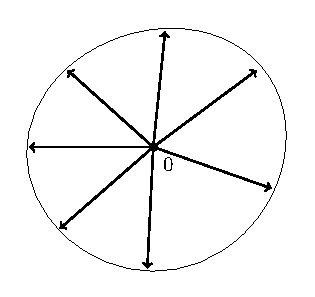
\includegraphics[scale=0.8]{figures/tikz/star_domain.pdf}
\caption{Darstellung eines Sterngebietes}
\end{figure}
\begin{lem}[Differential der Exponentialabbildung]
Wir wissen bereits: $\expp: \covd_p  \longrightarrow \mfk$ sowie $\expp_p(0) = p $. \\
Für das Differential der Exponentialabbildung ergibt sich dann:
\begin{align*}
\dd(\expp_p): T_0T_p\mfk &\longrightarrow T_p\mfk \\
v &\longmapsto v
\end{align*}
das heißt $\dd(\expp_p)_0=\operatorname{id}$.
\end{lem}
\begin{bew}
\begin{align*}
\dd(\expp_p)_0(v) &= \eval{\frac{\dd}{\dd t}}_{t=0} \expp_p(0+t\cdot v)  \\
&= \eval{\frac{\dd}{\dd t}}_{t=0}c_{t\cdot v}(1) \\
&= \eval{\frac{\dd}{\dd t}}_{t=0}c_v(t) \\
&= c_v(0) \\
&=v
\end{align*}
\end{bew}

\begin{kor}
Für alle $p \in \mfk$ existiert eine Umgebung $U$ von $0 \in T_p\mfk$ und eine Umgebung $V$ von $p \in \mfk$, so dass $\expp_p: U \longrightarrow V$ \ ein Diffeomorphismus ist.
\end{kor}
\missingfigure{Exponentialabbildung}

Falls $(\mfk, \nabla)$ vollständig ist, dann ist die Exponentialabbildung auf ganz $T\mfk$ definiert. \\
Wir haben gesehen: 
\begin{align*}
(S^n, g): c_v(t) = \cos(\norm{v}t) p + \sin(\norm{v}t)\frac{v}{\norm{v}}
\end{align*}
Falls $\norm{v}=2\pi$, dann gilt:
\begin{align*}
\expp_p(v) = c_v(1)=p
\end{align*} 
Daraus folgt, dass $\expp$ nicht injektiv ist, also damit auch kein globaler Diffeomorphismus. \\
\phantom{.} \\
Wir wollen nun wieder zurück zur Behandlung der Geodätischen kommen. Besonders interessieren wir uns jetzt für eine spezielle Eigenschaft der Geodätischen, nämlich dass die Geodätische längenminimierende Kurven sind. \\
Es sei $(\mfk, g)$ eine Riemannsche Mannigfaltigkeit und $c:[a, b] \longrightarrow \mfk$ eine glatte Kurve.
\begin{defs}[Länge einer Kurve c]
\begin{align}
L(c) &= \int_{a}^{b}\sqrt{(g(\dot{c}(t), \dot{c}(t))} \dd t  \nonumber \\
&= \int_{a}^{b} \norm{\dot{c}(t)} \dd t
\end{align}
\end{defs}
\begin{defs}[Energie von c]
\begin{align}
E(c) &= \frac{1}{2}\int_{a}^{b}(g(\dot{c}(t),\dot{c}(t))) \dd t \\
&= \frac{1}{2}\int_{a}^{b} \norm{\dot{c}(t)}^2 \dd t
\end{align}
\end{defs}

\begin{bem}
Die Länge der Kurve ist unabhängig von der Parametrisierung:
\begin{align}
L(c) = L(c \circ \varphi)
\end{align}
für Umparametrisierungen:
\begin{align*}
\varphi: [a, b] \longrightarrow [\tilde{a}, \tilde{b}]
\end{align*}
\missingfigure{kleine Skizze Koordinatensystem}
\end{bem}
\begin{bew}
\begin{align*}
L(c \circ \varphi) &= \int_{a}^{b} \norm{\frac{\dd}{\dd t} (c \circ \varphi)(t)} \dd t \\
&= \int_{a}^{b} \norm{\dot{c}(\varphi(t))} \dot{\varphi}(t) \dd t \quad ;\dot{\varphi}(t) > 0 \\
&= \int_{\tilde{a}}^{\tilde{b}} \norm{\dot{c}(s)} \dd s \\
&= L(c)
\end{align*}
wobei $s=\varphi(t)$.
\end{bew}
\begin{bem}
Die Energie hängt von der Parametrisierung ab!
\end{bem}
\begin{lem}
Es gilt die Ungleichung:
\begin{align}
L(c)^2 \leq 2(b-a)E(c)
\end{align}
wobei Gleichheit genau dann gilt, wenn $c$ proportional zur Bogenlänge parametrisiert ist.
\end{lem}
Seien nachfolgend $p, q \in \mfk$. 
\begin{align*}
\Omega_{p, q} = {\text{stückweise glatte Kurven von p und q}}
\end{align*} 
\missingfigure{Darstellung stw. glatte Kurven}
\begin{align*}
L: \Omega_{p, q} \longrightarrow \R
\end{align*}
Variation:
\begin{figure}[H]
\centering
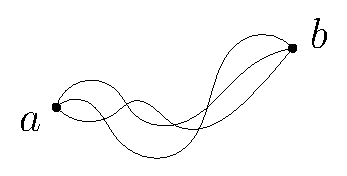
\includegraphics[width=0.35\linewidth]{figures/tikz/variation.pdf}
\caption{Variation einer Kurve mit festem Anfangs- und Endpunkt.}
\label{img:variation}
\end{figure} 
Betrachten wir eine $1$-Parameter Familie von Kurven:
\begin{align*}
I \ni s |\longrightarrow c_s \in \Omega_{p, q}
\end{align*}
so dass $L(c_s)$ glatt von s abhängt.
\begin{align*}
\partial_s\eval{L(c(s))}_{s=0} = 0 \  \longleftrightarrow \ c \quad \text{Geodätische}
\end{align*}

\begin{defs}[1-Parameter Variation]
Eine stückweise glatte $1$-Parameter Variation von $c:[a, b] \rightarrow \mfk$ ist eine Abbildung
\begin{align*}
\mathcal{H}: I \times [a, b] &\longrightarrow \mfk \\
(s, t) &\longmapsto \mathcal{H}(s, t)
\end{align*}
Mit $\mathcal{H}(0, t) = c(t)$ genau so, dass 
\begin{align*}
a= t_0 \leq t_1 \leq \cdots \leq t_m = b
\end{align*}
existiert, wobei $\mathcal{H}$ glatt auf $I > [t_i, t_{i+1}]$ ist.
\begin{figure}[H]
\centering
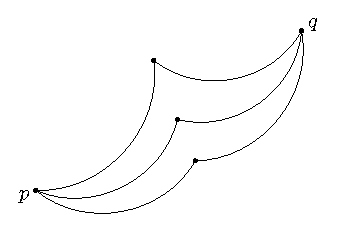
\includegraphics[width=0.45\linewidth]{figures/tikz/variationpiecewise.pdf}
\caption{Variation einer stückweise glatten Kurven vom Punkt $a$ nach $b$.}
\label{img:variationpiecewise}
\end{figure}
Eine solche Variation heißt \textbf{eigentlich}, falls:
\begin{align*}
\mathcal{H}(s, a) &= c(a) \\
\mathcal{H}(s, b) &= c(b) 
\end{align*}
\end{defs}
Wir setzen $c_s = \mathcal{H}(s, \cdot)$ sowie $c_0 = c$. \\
Das Variationsfeld von $\mathcal{H}$ ist:
\begin{align*}
V(\cdot) = \partial_s \mathcal{H}(0,\cdot) = \eval{\partial_s \mathcal{H}(s, \cdot)}_{s=0}
\end{align*}
$V$ ist ein stückweises Vektorfeld längs $c$. \\
$\mathcal{H}$ ist eigentlich $\Rightarrow \ V(a) = V(b) = 0$.
\missingfigure{Aussehen des Vektorfelds}
\begin{lem}
Sei $c:[a, b] \longrightarrow \mfk$ eine stückweise glatte Kurve und $V$ ein stückweise glattes Vektorfeld längs $c$. 
Dann existiert eine $1$-Parameter Variation $\mathcal{H}: I \times [a, b] \longrightarrow \mfk$ von $c$ mit Variationsfeld $V$ und $\mathcal{H}(s, t) = c(t) \ \forall t$ für die $V(t)=0$.
\end{lem}
\begin{bew}
\begin{align*}
\mathcal{H}(s, t) = \expp_p{c(t)}(s(V(t)))
\end{align*}
\end{bew}
\begin{figure}[H]
\centering
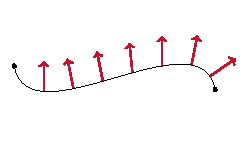
\includegraphics[width=0.45\linewidth]{figures/tikz/variation_field.pdf}
\caption{Darstellung des Variationsfeldes}
\label{img:variation_field}
\end{figure}
\begin{satz}
Sei $c:[a, b] \longrightarrow \mfk$ proportional zur Bogenlänge parametrisiert. \\
Sei $\mathcal{H}: I \times [a, b] \longrightarrow \mfk$ eine stückweise glatte $1$-Parameter Variation von c, $V$ das Vektorfeld $V=\partial_s\mathcal{H}(0,\cdot), c_s=\mathcal{H}(s,\cdot)$ und $L(s) = L(c(s))$. \\
Dann ist $L: I \longrightarrow \R$ glatt um $0 \in I$ und die erste Ableitung $\partial_sL(0)$ ist gegeben durch:
\begin{align*}
\partial_sL(0) = \frac{1}{\norm{\dot{c}(t)}}\left[\eval{g(V,\dot{c})}_{a}^{b} + \sum_{i=0}^{n-1}g(V(t_i),\Delta\dot{c}(t_i))- \int_{a}^{b}g(V,D_t\dot{c})\dd t\right]
\end{align*}
Hierbei gilt $a=t_0 \leq \cdots \leq t_m=b $ und 
\begin{align*}
\Delta\dot{c}(t_i) = \underbrace{\dot{c}(t_i-0)}_{\text{von links}} - \underbrace{\dot{c}(t_i+0)}_{\text{von rechts}}
\end{align*}
\end{satz}
Die Notation bedeutet, dass die Kurve stückweise glatt ist und die Ableitung an den Verbindungpunkten  springt. Wir haben also zwei verschiedene Grenzwerte.
\begin{bem}
Vor dem Beweis des vorangegangen Lemmas wollen wir noch einige Bemerkungen machen:
\begin{enumerate}
\item $\partial_sL(0)$ hängt nur von $V$ ab und nicht explizit von $\mathcal{H}$.
\item $c$ glatt $\Rightarrow$ Term $\Delta\dot{c}(t_i)=0$.
\item $c $ Geodätische $\Leftrightarrow \covd_t\dot{c} = 0$ .
\end{enumerate}
\end{bem}
\begin{bew}[Vorangegangenes Lemma]
\begin{align*}
L(s) = \sum_{i=0}^{n-1} \int_{t_i}^{t_i+1}\norm{\dot{c}_s(t)} \dd t \quad \text{ist glatt in $s$.}
\end{align*}

Berechne die Ableitung:
\begin{align*}
\partial_sL(0) &= \frac{\dd}{\dd s}\eval{\left[\sum \int \norm{\dot{c}_s(t)} \dd t\right]}_{s=0} \dd t \\
&= \sum \int \frac{\dd}{\dd s} \eval{\norm{\dot{c}_s(t)}}_{s=0} \dd t \\
&= \sum \int \frac{\dd}{\dd s} \eval{\sqrt{g(\dot{c}_s(t),\dot{c}_s(t))}}_{s=0} \dd t \\
&= \sum \int \frac{1}{2} \frac{1}{\norm{\dot{c}(t)}}\frac{\dd}{\dd s}\eval{g(\dot{c}_s(t),\dot{c}_s(t))}_{s=0} \dd t \\
&=\frac{1}{\norm{\dot{c}(t)}}\sum\int\frac{1}{2}\cdot 2\eval{g(\covd_s\dot{c}_s(t),\dot{c}_s(t))}_{s=0} \dd t \\
&=\frac{1}{\norm{\dot{c}(t)}}\sum\int g(\covd_s \frac{\dd}{\dd t}\mathcal{H}(s, t), \frac{\dd}{\dd t} \mathcal{H}(s, t)) \dd t \\
&=\frac{1}{\norm{\dot{c}(t)}}\sum\int g(\covd_t \frac{\dd}{\dd s}\mathcal{H}(s, t), \frac{\dd}{\dd t} \mathcal{H}(s, t)) \dd t \\
&=\frac{1}{\norm{\dot{c}(t)}}\sum\int g(\covd_tV, \dot{c}(t)) \dd t \\
&=\frac{1}{\norm{\dot{c}(t)}}\sum\int \left(\frac{\dd}{\dd t}g(v(t), \dot{c})-g(v(t),\covd_t\dot{c}(t))\right) \dd t
\end{align*}
\end{bew}
